%************************************************
\chapter{Conclusion}\label{ch:conclusion} % $\mathbb{ZNR}$
%************************************************

Neuronal networks must produce stable circuit output for sustained periods of time despite environmental perturbation. In addition, they must be sensitive to key endogenous signaling to produce differing output. The \acs{STG} manages these competing objectives while remaining degenerate to ion channel density. Neuromodulators can produce a diverse set of network states using the same cellular and synaptic morphology. In particular to the \acs{STG}, the dense, tangled neuropil and gradations in reversal potential render neurons isopotential with respect to the somata. Neuromodulators, then, play the role of maintaining and switching network activity. 

Many neuromodulators, such as proctolin and \acs{RPCH} activate an inward mixed-cation \ac{IMI}. This current drives the network by activating near the spiking threshold. Networks with \acs{IMI} experience more stable, faster rhythms in comparison to decentralized states.

The \acs{STG} database demonstrated cellular and network degeneracy with respect to maximal conductances, but did not incorporate the effects of modulation. Only a small subset of Prinz models respond to modulatory input (\autoref{fig:prinzburstingmodelsnavcatswensen}). Optimization by gradient descent produced a set of single-compartment \acs{AB} models which increase in frequency slowly as a function of modulatory input maximal conductance (\autoref{fig:figprinzburstingttxcatnoscgmiswensenexprosim3}). Amplitude of these oscillations shifted from sub-threshold (< 20 mV) to high amplitude (> 20 mV) over a small range of modulatory input. Within these two regimes, the amplitude did not strongly depend on modulatory input. These data indicate that the models undergo amplitude transition with modulatory input switching the model between these qualitative states.

Using particle swarm optimization, models were simulated over a smaller range of \acs{IMI} maximal conductance (\autoref{fig:abwmod}). At low maximal conductance, \acs{AB} models increase in frequency and amplitude as a smooth function of \acs{IMI}. Over larger ranges of maximal conductance, models converge to the sharp increase. These results recapitulate dose-responser curve data at low concentrations of oxotremorine (D. Hampton, unpublished) and \acs{RPCH}\autocite{NusbaumNeuronalRoleCrustacean1988}.

\begin{figure}
	\centering
	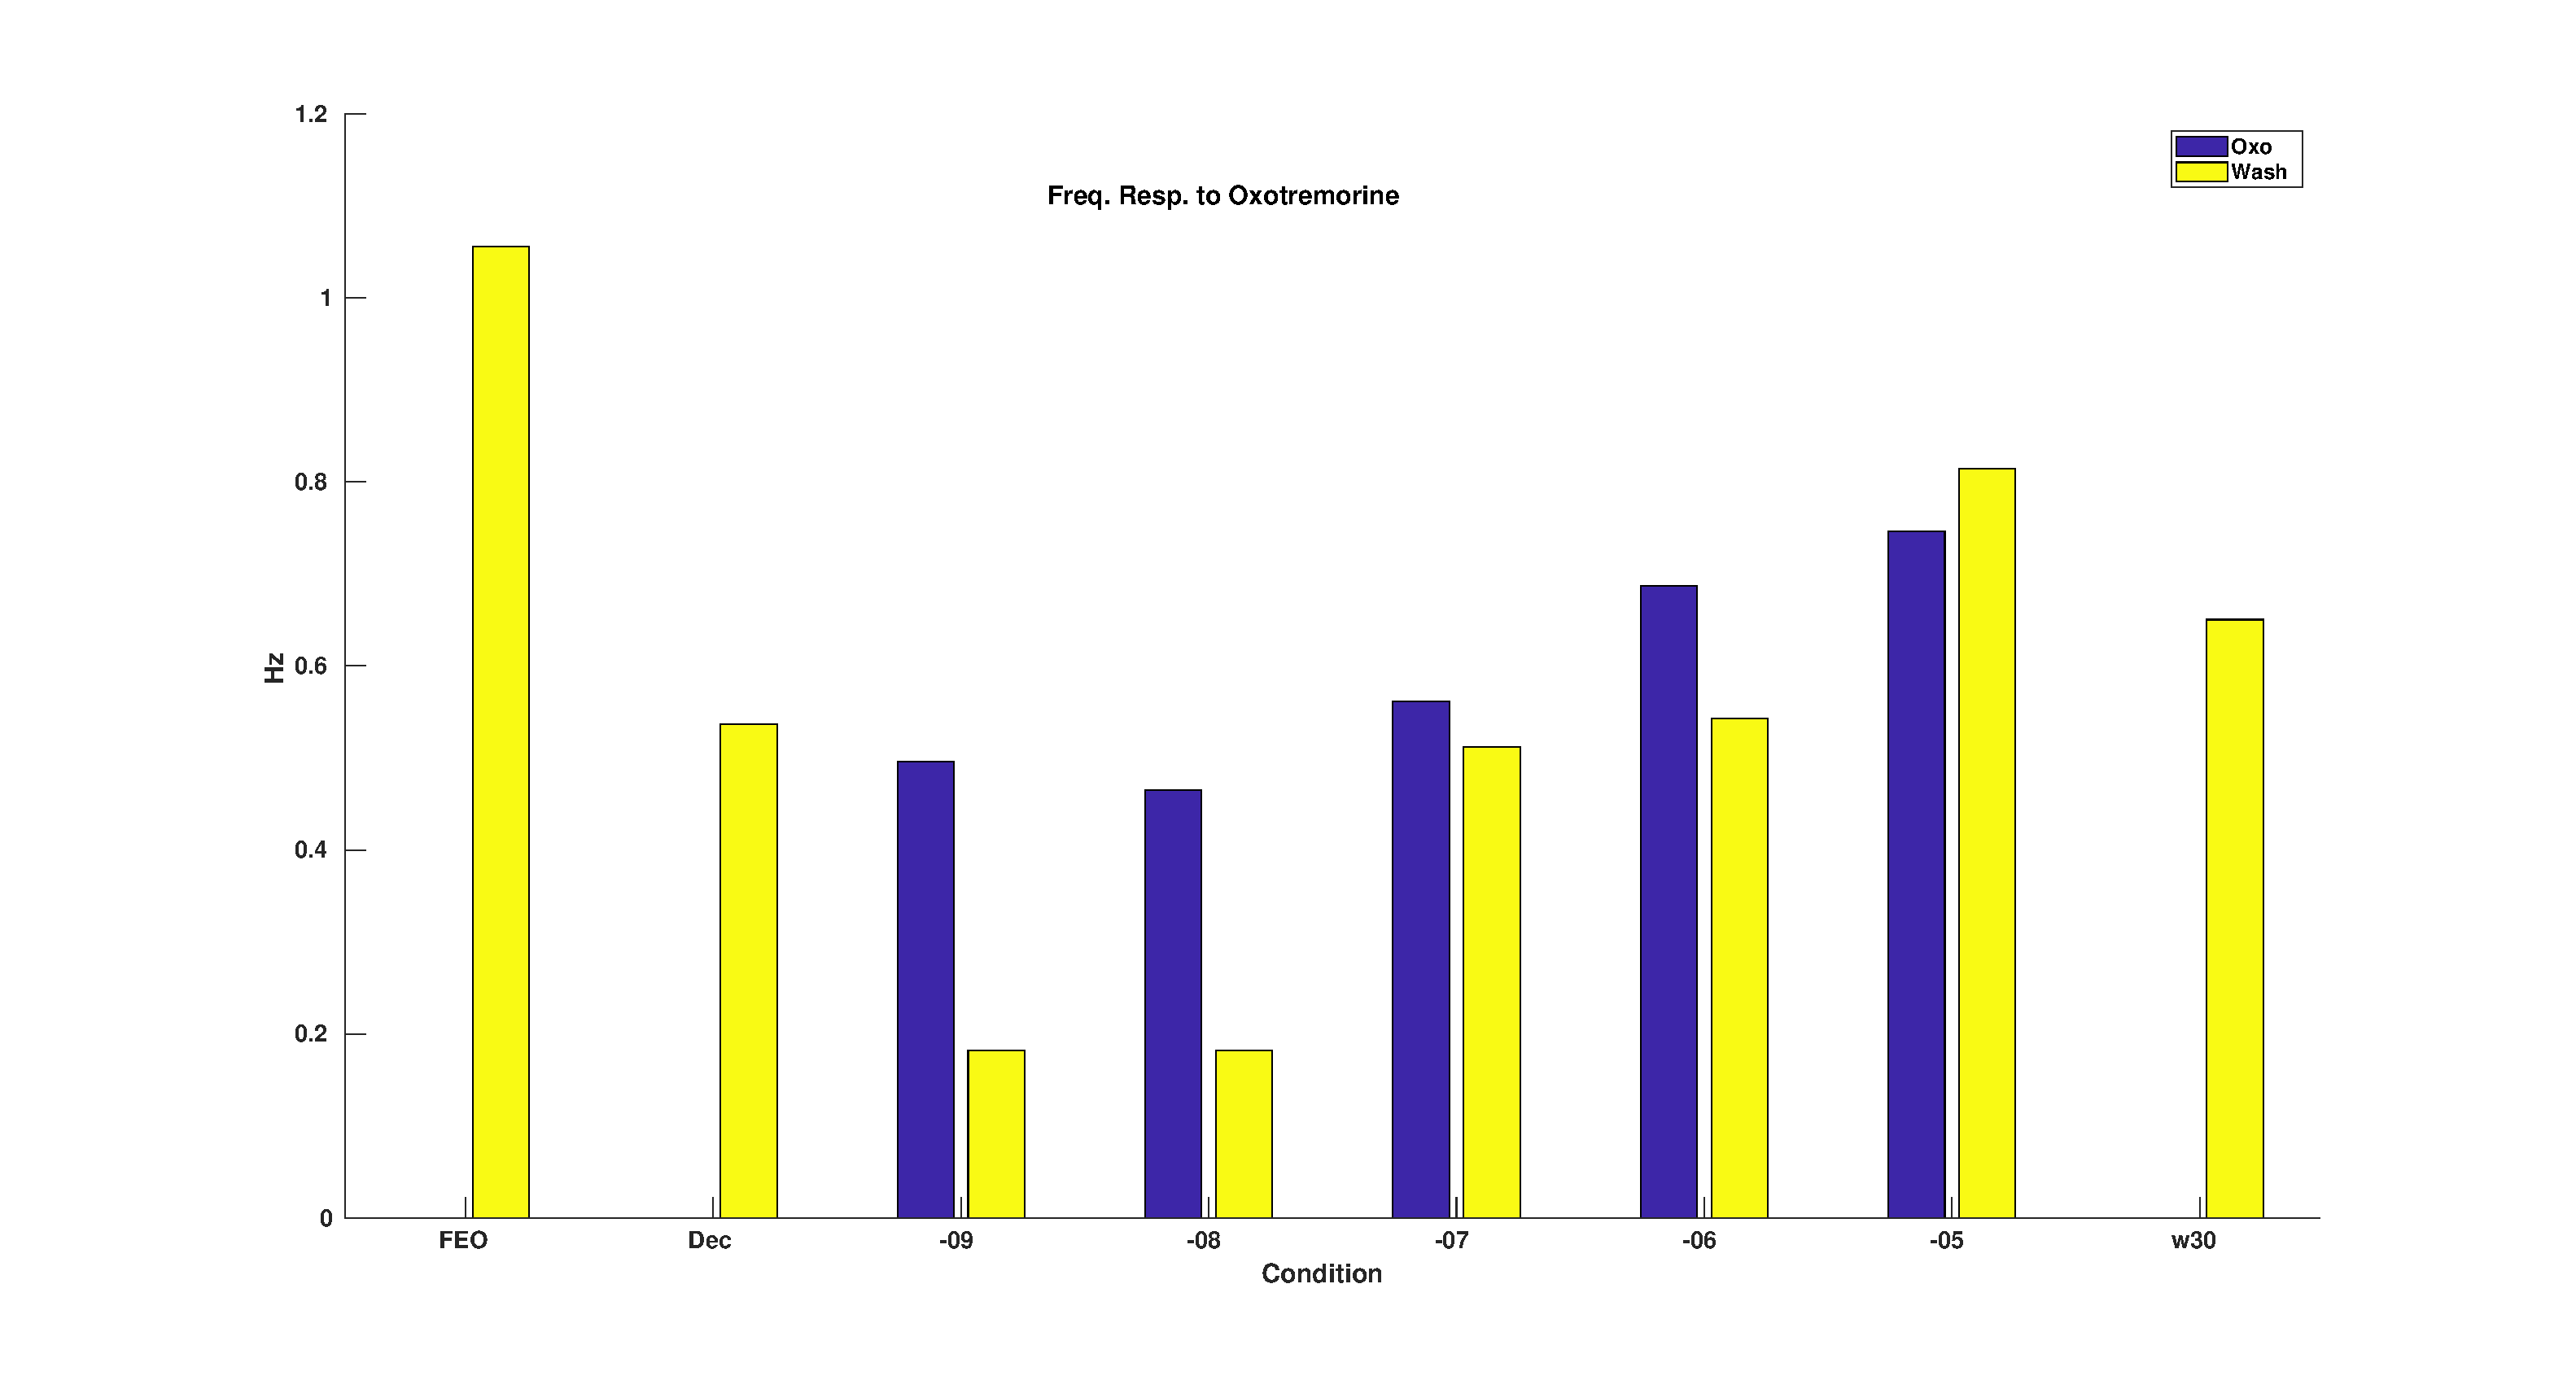
\includegraphics[width=1.0\linewidth]{gfx/Oxo_Dose_Resp_curve}
	\caption[Burst frequency dose response to oxotremorine]{Burst frequency dose response to oxotremorine at low concentration demonstrates increasing response to modulatory input (D. Hampton, unpublished). Yellow bars indicate wash in physiological saline, blue indicates presence of oxotremorine in logarithmic molar concentration.}
	\label{fig:oxodoserespcurve}
\end{figure}


Optimization of network models demonstrated \acs{IMI} in single compartment network models. While network models in this form have been shown to be degenerate with respect to ionic and synaptic maximal conductances\autocite{PrinzAlternativehandtuningconductancebased2003,PrinzSimilarnetworkactivity2004,PrinzComputationalapproachesneuronal2010}, robustness to modulatory input has not been well studied. In basal conditions, network models received modulatory input into \acs{AB}-\acs{PD}, \acs{LP}, or both. When modulatory input was removed, burst frequency and amplitude decreased (\autoref{fig:networkab47traces}), and some models lost triphasic rhythmicity (\autoref{fig:networkablp14traces}, \autoref{fig:networklp28traces}). These examples demonstrate the power of particle swarm optimization to produce models which fit arbitrary constraints. Single-compartment three-cell networks are capable of reproducing the neurocomputational effects of modulation on the pyloric rhythm.

When optimization protocols did not favor any particular modulation state (\acs{AB}-\acs{PD}, \acs{LP}, or both), modulation into \acs{AB}-\acs{PD} and \acs{LP} was revealed to be the most reliable method to initiate pyloric rhythmicity from a non-triphasic network, and increase burst frequency and slow wave amplitude in triphasic, decentralized networks (\autoref{fig:allstats}). \acs{AB} cells near transitions to tonic firing or depolarization block are uncommon \textit{in-vitro}. Models near these points in parameter space tend to increase in burst frequency with \acs{IMI} in \acs{LP} (\autoref{fig:traces3}) and transition out of triphasic activity with modulation into \acs{AB}-\acs{LP} (\autoref{fig:traces4}).

Of triphasic networks with pacemaker kernels robust to external depolarization and hyperpolarization, none showed increased burst frequency and amplitude during \acs{LP} modulation with respect to the decentralized condition (\autoref{fig:allstats}). These models display qualitatively similar activity to experimental results with \acs{CCAP}\autocite{WeimannModulationOscillatorInteractions1997}. Modulation onto \acs{LP} provides antiphase hyperpolarization to \acs{PD}. In conjunction with \acs{IMI} in \acs{AB}-\acs{PD}, \acs{RPCH} and other neuromodulators drive robust pyloric rhythmicity.

Correlations between maximal conductances in cases where networks are non-pyloric in decentralized conditions and pyloric under neuromodulation against control conditions pyloric everywhere. Networks which became pyloric under neuromodulation tended to have lower calcium conductances (\autoref{fig:correlationsab}). In addition, \acs{LP} models tuned \acs{IKCa} to \acs{IH}. These relationships indicate strong potential for post-inhibitory rebound-mediated bursting. The results provide support for \acs{AB}-\acs{PD} as pacemaker that drives \acs{LP} and \acs{PY}. Modulation of \acs{PY} is likely less necessary because of the many electrically coupled neurons and half-center connection to \acs{LP}. \acs{PY} can readily generate trains of action potentials down descending axons when inhibited rhythmically by \acs{AB}, \acs{PD}, and \acs{LP}. 

These investigations were motivated by P. Rosenbaum's experiments in \acs{TTX} and \acs{RPCH} which demonstrated stereotyped rhythmic oscillations unique to each preparation. Rhythmic activity with periods on the order of 5-10 s were observed. This timescale is vastly longer than intrinsic dynamics of any currents contributing to the change in membrane potential. Computational work endeavored to propose a hypothesis for these phenomena.

\begin{figure}[h]
	\centering
	\includegraphics[width=1.0\linewidth]{gfx/RPCH_TTX_real_data}
	\caption[Long timescale oscillations in RPCH and TTX]{Start of \acs{RPCH}-\acs{TTX} rhythm. No rhythmic activity in \acs{TTX}, but after application of \acs{RPCH} rhythms start A, with large amplitude, slow frequency oscillations in both \acs{PD} and \acs{LP} predominantly large amplitude slow frequency oscillations. Vertical scale bars denote 10 mV, horizontal scale bars membrane potential at -50 mV (P. Rosenbaum, unpublished).}
	\label{fig:rpchttxrealdata}
\end{figure}

\begin{figure}[h]
	\centering
	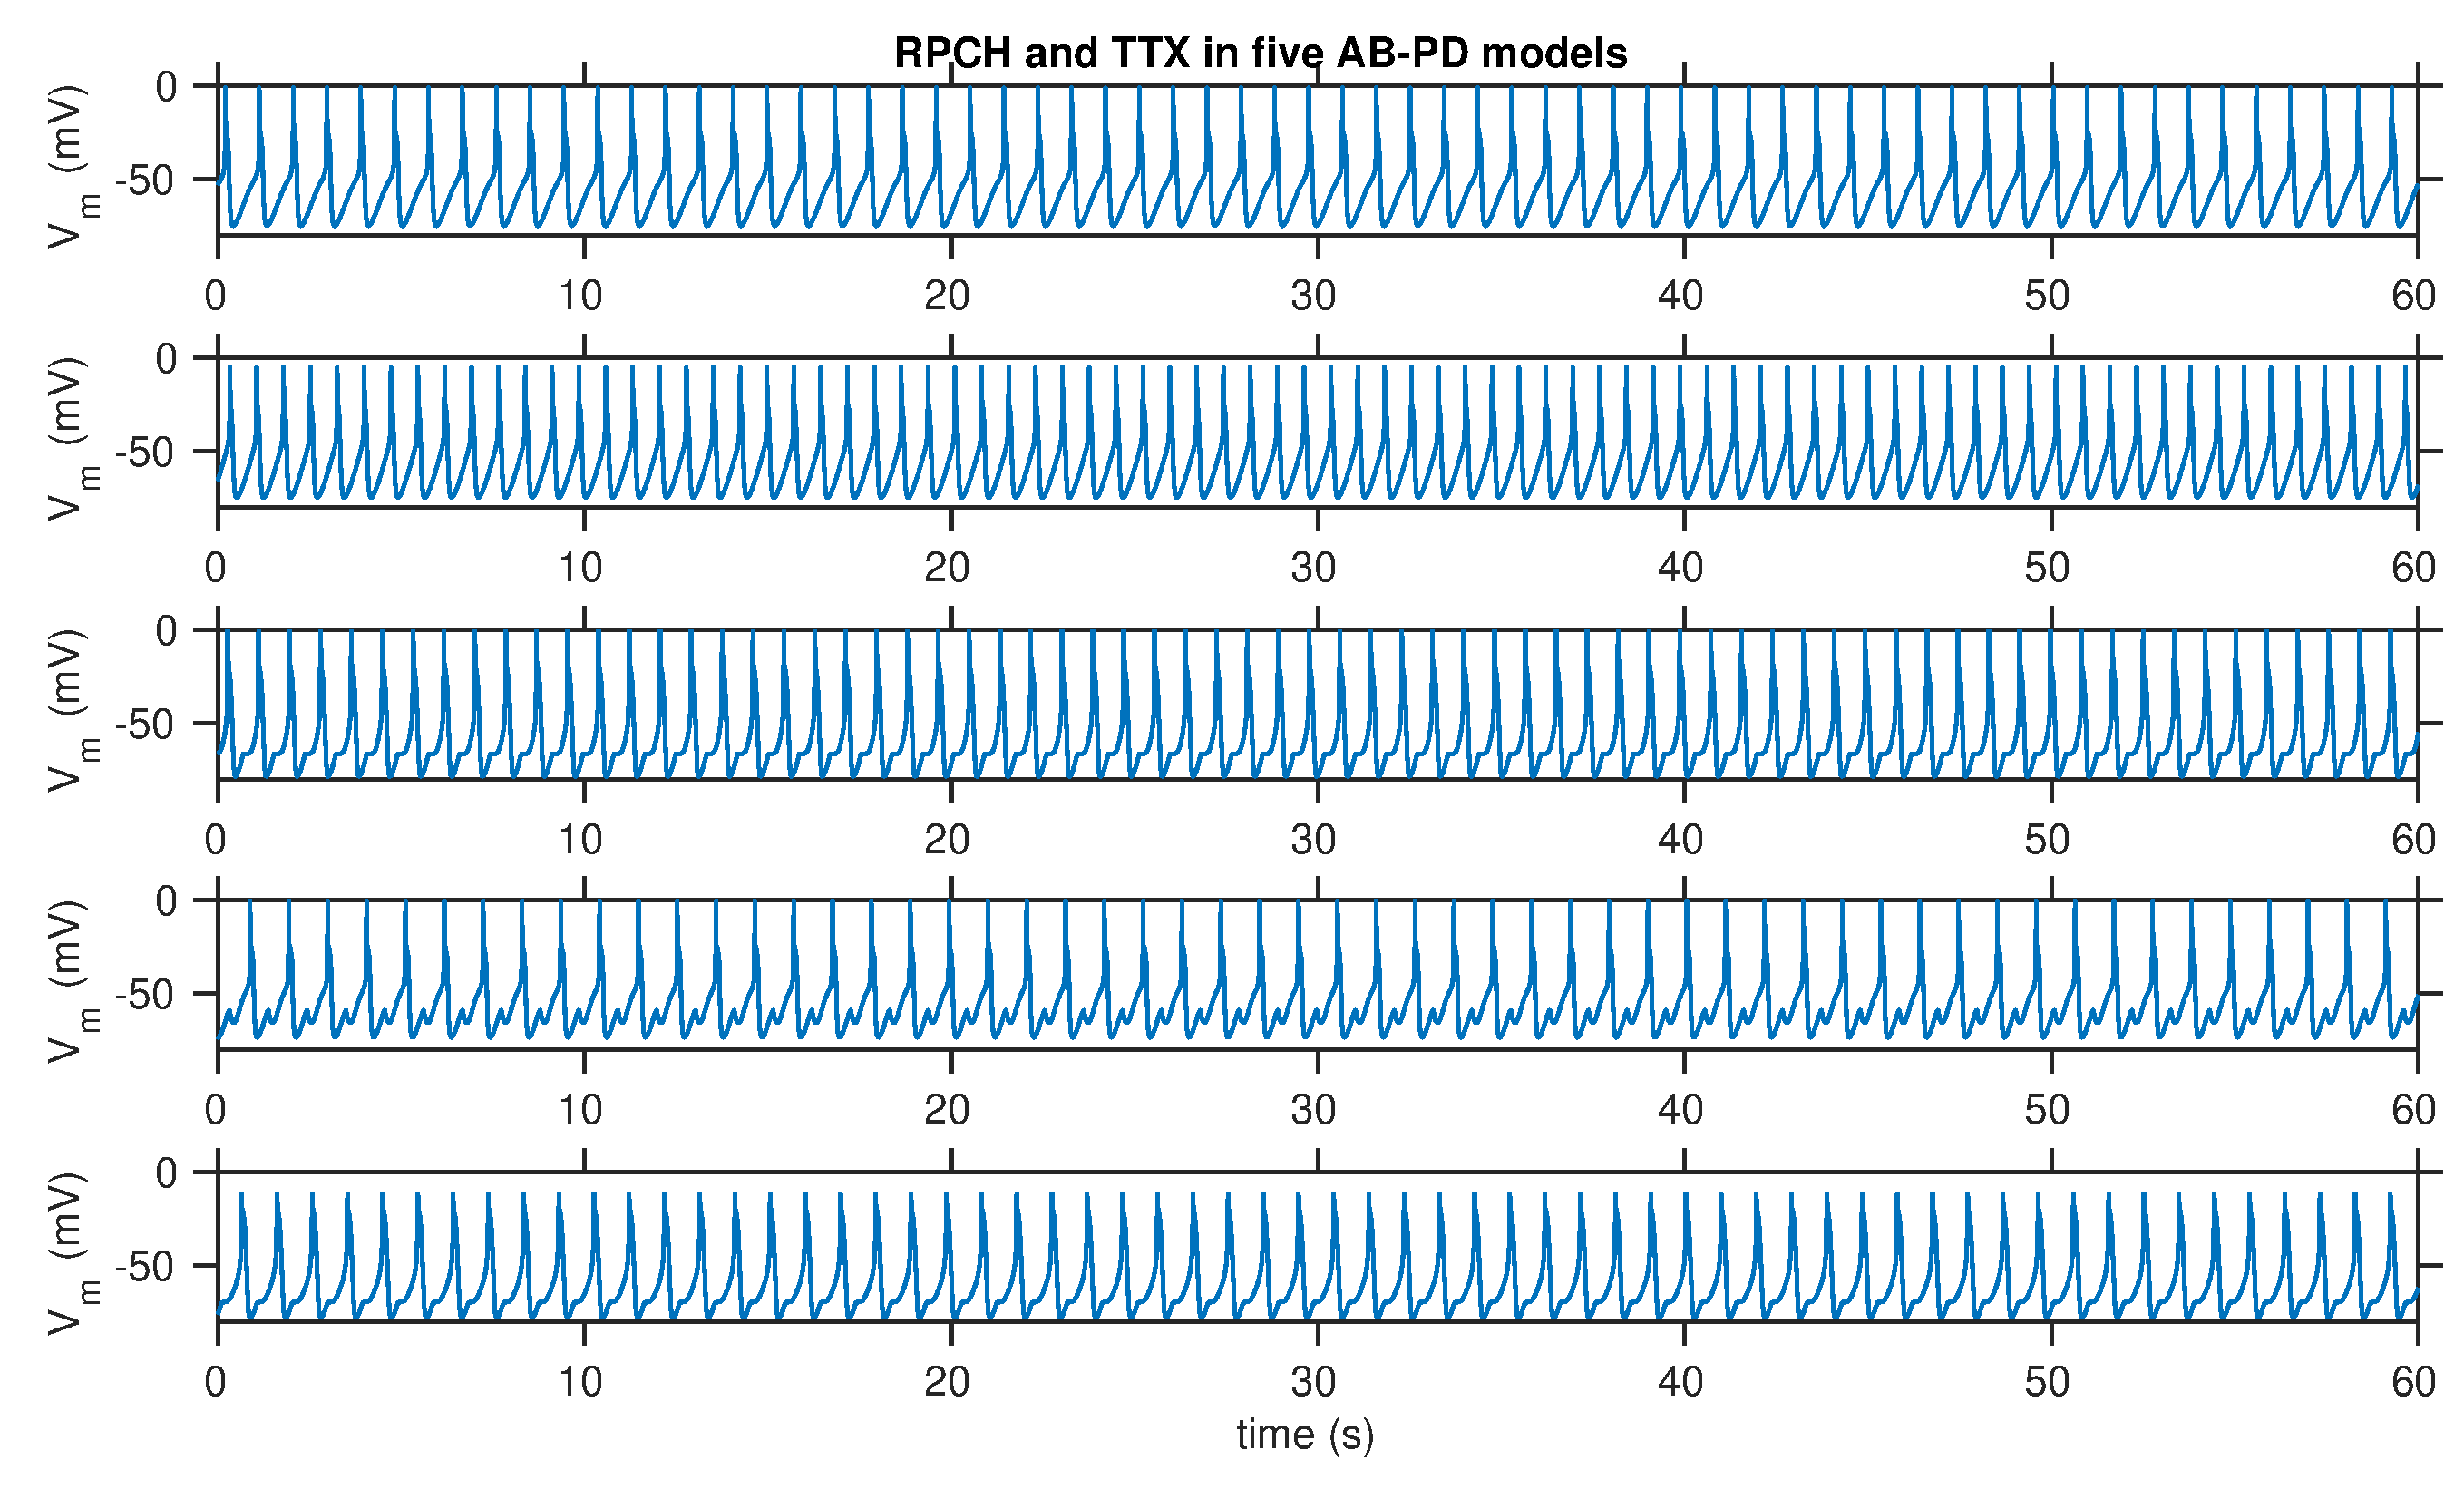
\includegraphics[width=1.0\linewidth]{gfx/RPCH_TTX}
	\caption[RPCH and TTX in optimized AB-PD models]{\acs{RPCH} and \acs{TTX} in \acs{AB}-\acs{PD} models produces rhythmic activity. Simulated data are asymptotically stable, without phenomena on timescales > 2 s. Graded synaptic transmission maintains triphasic rhythm in the absence of sodium spikes.}
	\label{fig:rpchttx}
\end{figure}

\FloatBarrier

The three cell model does not, at this time, account for any effects on timescales > 2 s. When additional cells contributing to the pyloric network were added (viz. \acs{IC}, \acs{VD}), plateau potentials emerged in \acs{LP} at timescales > 5 s. In order to develop a model that recapitulates the underlying variability revealed by \acs{RPCH} and \acs{TTX}, a more complete model of the pyloric circuit must be developed. In the current timescale, this thesis demonstrates that single-compartment three-cell network models of the pyloric rhythm are sufficiently complex to reproduce the effects of \acs{IMI}. The models maintain the maximal conductance degeneracy of previous work, while demonstrating robustness to modulatory input. The simulation environment \texttt{xolotl} and particle swarm optimization protocols are ready to be implemented on larger scale endeavors.




%*****************************************
%*****************************************
%*****************************************
%*****************************************
%*****************************************
